\documentclass[11pt]{article}
\usepackage{geometry}
\geometry{letterpaper, margin=1in}
\usepackage[utf8]{inputenc}
\usepackage{graphicx}
\usepackage{upgreek}
\usepackage{url}
\usepackage[T1]{fontenc}
\usepackage{amsmath}
\usepackage{minted}
\usepackage{scalerel}
\usepackage{multicol}
\usepackage[colorinlistoftodos]{todonotes}
\usepackage[
backend=biber,
style=ieee, 
sorting=none
]{biblatex}
 
\addbibresource{refs.bib}

\title{ECE532S Digital Systems Design \\ \vspace{0.4cm}
       \Large Tutorial 2 - Creating a Simple MicroBlaze Project \\ \vspace{0.4cm}
       \small Last Updated: July, 2019}
\author{ }
\date{ }


\begin{document}
\maketitle
\vspace{-1cm}

\textit{Soft processors}, such as MicroBlaze, are implemented using programmable logic (FPGA LUTs and registers) and can be custom configured to suit the software application they run. In contrast, \textit{hard processors}, such as the Intel i7 CPU, are implemented as application-specific integrated circuits (ASICs), and their functions are fixed after manufacture. Soft processors are common in embedded systems built with FPGAs, and they usually provide high-level control logic for the system. They can be quickly and easily programmed with a C-based language, and have the advantage of customization. For example, the user can choose between various instruction and data caches, as well as choose to include custom instructions for faster execution of an application. In short, a \textit{soft processor} is a parameterizable processor core that can be built within the logic of an FPGA. 

In this tutorial, we will build a simple MicroBlaze-based soft-processor system on the Nexsys DDR FPGA. The MicroBlaze system we build will be composed of the following Xilinx IP:

\begin{multicols}{2}
\begin{itemize}
    \item MicroBlaze Processor
    \item AXI Timer
    \item UARTLite
    \item Debug Module (MDM)
    \item Processor System Reset
    \item Interrupt Controller
    \item Local memory bus (LMB)
    \item Clock Wizard
\end{itemize}
\end{multicols}

\noindent
These are the basic building blocks used in a typical MicroBlaze system. In addition to creating the system described above, this tutorial also describes the development of a small application that we develop within the Xilinx Software Development Kit (SDK) in the Vivado Design Suite. The application code developed in the SDK prints “Hello World” on a terminal.




\section{Creating a Vivado Project with a Block Design}
\label{sec:create_proj}
Invoke the Vivado IDE to create a new project as described in Tutorial 1. From the \textit{Getting Started} page, select \textbf{Create New Project}. In the \textit{Project Name} dialog box, type the project name and location; make sure to choose a directory to which you extracted the contents of the provided \textit{zip} file for this tutorial. In the \textit{Project Type} dialog box, select \textbf{RTL Project}. In the \textit{Add Sources} dialog box, ensure that the Target language is set to \textbf{Verilog}; we don't have any source to add to this project. In the \textit{Add Constrains and Add Existing IP} dialog box make sure to \textbf{Add} the \textit{microblaze.xdc} constraints file included in the tutorial \textit{zip} file. Choose \textbf{xc7a100tcsg324-1} in the \textit{Default Part} dialog box. Click \textbf{Finish} to finish creating the project.

Next, we will create a new \textit{Block Diagram} for our MicroBlaze system. Select \textbf{Create Block Design} under the \textit{IP Integrator} section of the \textit{Flow Navigator} pane. Specify any design name and click \textbf{OK} to finish the creation of the block diagram. Once the block design has been created, you should see the interface presented in Figure~\ref{fig:block_design_blank}. Block Designs are an alternate way to design a hardware system in the Vivado IDE, presenting a graphical interface where various IPs and Verilog source files can be connected using \textit{click-and-drag} motions rather than typing out the connectivity in the Verilog code. Note, block diagrams are used by Vivado to generate Verilog.

\begin{figure}[h]
    \centering
    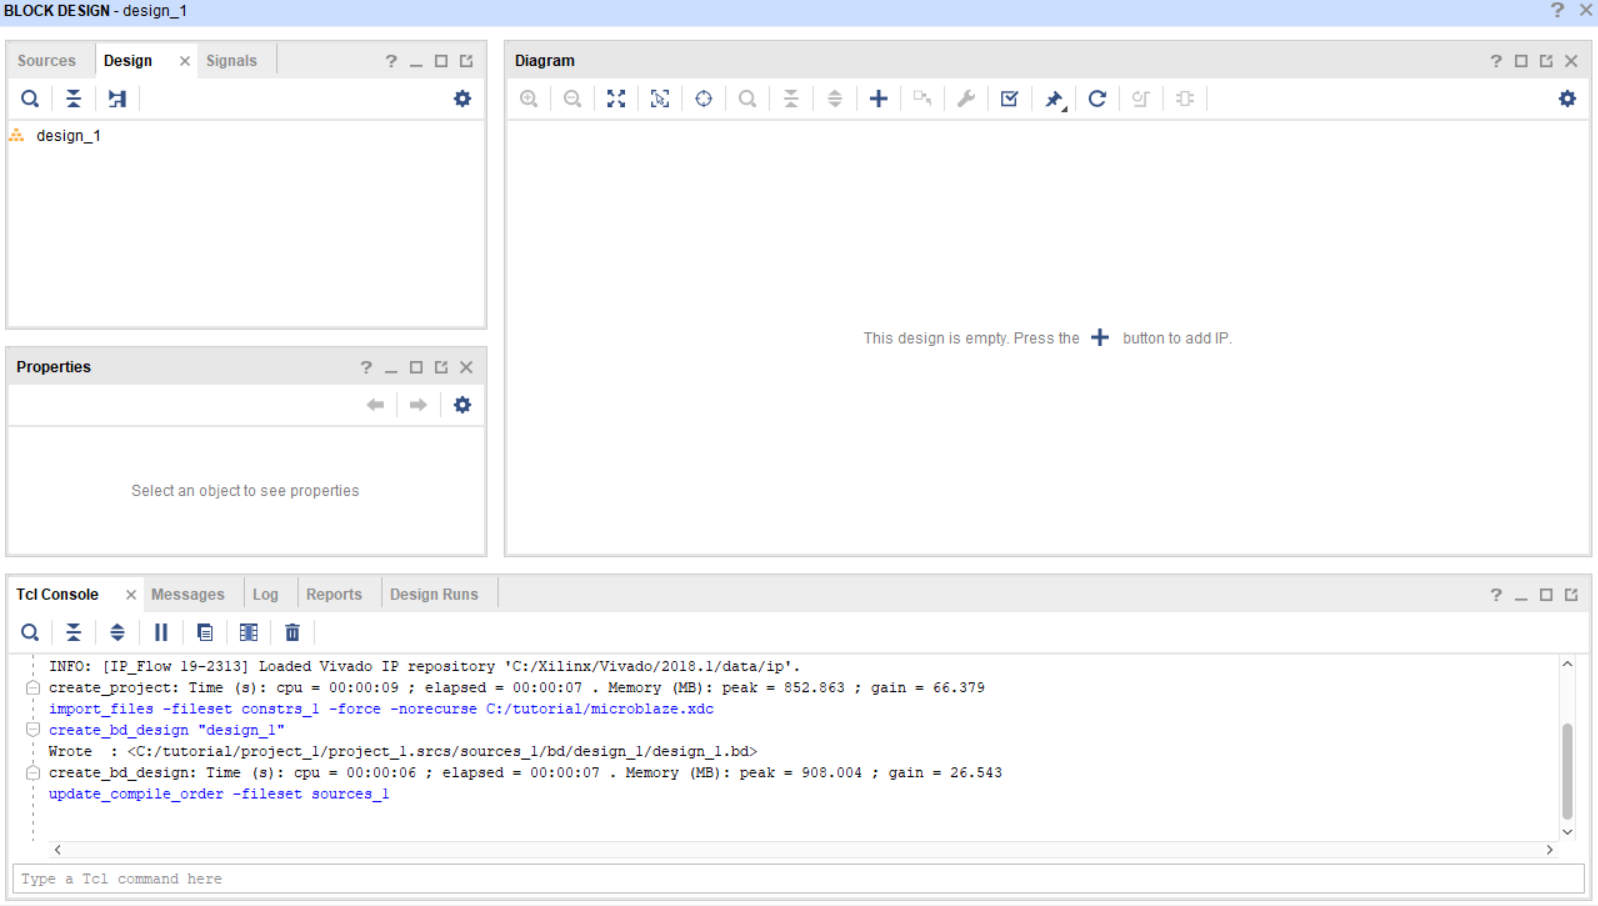
\includegraphics[width=0.9\textwidth]{images/block_design_blank.png}
    \caption{The Block Design editor view}
    \label{fig:block_design_blank}
\end{figure}




\section{Creating a MicroBlaze System}
\label{sec:adding_cores}
Now that we have a blank block design created, we need to add the IP cores for the functionality we hope to implement. The first IP Core we're going to add is the MicroBlaze soft-processor. Click the \textbf{Add IP}
(\scalerel*{
\includegraphics{images/add_ip.png}}{(})
button, either on the toolbar above the block diagram or in the middle of the block design field, to add an IP Core. You can also \textbf{Right Click} and select \textbf{Add IP} anywhere in the block diagram to add a new IP Core. In the Search field, type \textbf{microblaze} to find the MicroBlaze IP, then click \textbf{Enter}. Once the microblaze has been added, you should see a new Core within the Block Design, as depicted in Figure~\ref{fig:just_mb}.

\begin{figure}[h]
    \centering
    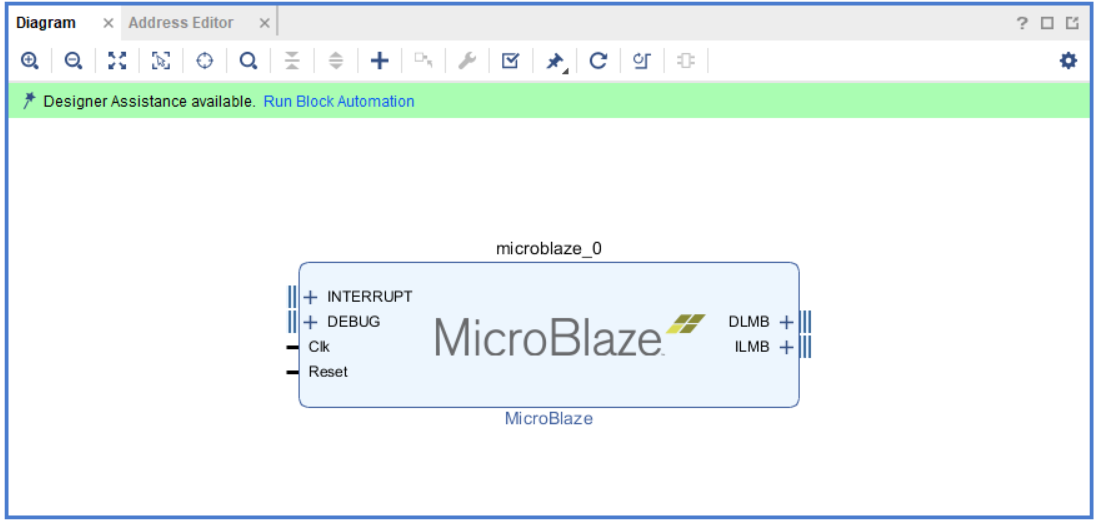
\includegraphics[width=0.9\textwidth]{images/just_mb.png}
    \caption{The Block Design with the newly added MicroBlaze IP}
    \label{fig:just_mb}
\end{figure}

\begin{figure}[!h]
    \centering
    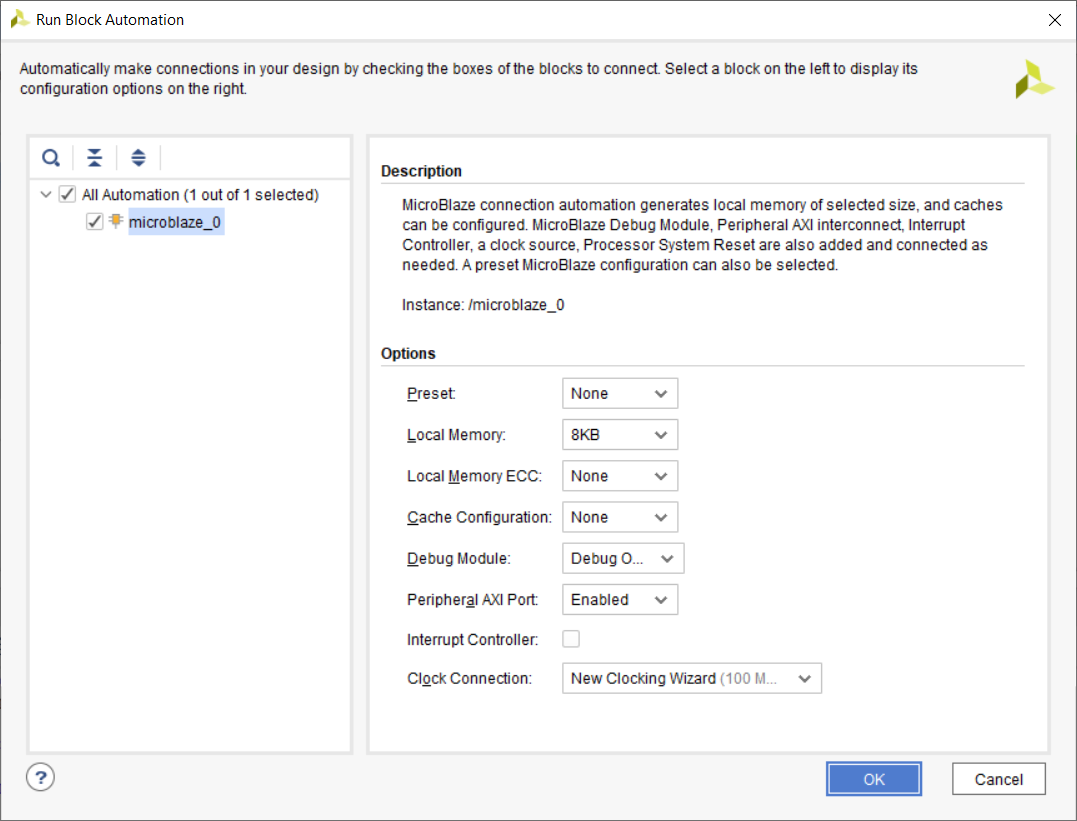
\includegraphics[width=0.9\textwidth]{images/block_auto.png}
    \caption{Block Automation wizard for the MicroBlaze IP}
    \label{fig:block_auto}
\end{figure}

We need to customize the MicroBlaze IP to our specific needs. In general, we can double-click on any IP in order to set its customization parameters. For some IPs, a feature called \textit{Block Automation} is provided which eases the selection of these parameters by only showing the most important parameters. Note, \textit{Block Automation} will also automatically instantiated (create) other IP Cores that are required in order to interface with the IP Core to be customized. We can take advantage of this feature to ease the creation of the full MicroBlaze system. Click the \textbf{Run Block Automation} link at the top of the Block Design to run \textit{Block Automation} (Note, this link is visible in Figure~\ref{fig:just_mb}).

The \textit{Block Automation} wizard you'll see is shown in Figure~\ref{fig:block_auto}. In the pane on the left side of the \textit{Block Automation} window is the list of IP Cores which are eligible for \textit{Block Automation}; here you can check/uncheck those blocks for which you want to run \textit{Block Automation}. Selecting an IP Core shows the set of customization parameters for that core in the pane on the right side. We should only see a single IP Core available for \textit{Block Automation}, the MicroBlaze IP, so select \textbf{microblaze\_0} (or whatever you're MicroBlaze happens to be named) on the left side. We see a couple of options to customize the MicroBlaze IP Core. From the pulldown menu, set \textit{Local Memory} to \textbf{32 KB}. Leave the \textit{Debug Module} option to its default state \textbf{Debug Only}. Leave the \textit{Peripheral AXI Port} option as \textbf{Enabled}. Check the \textbf{Interrupt Controller} option. Select the \textit{Clock Connection} option of \textbf{New Clocking Wizard (100 Mhz)}. This will create a clock signal in the block design for the MicroBlaze. Once you've set all these settings, click \textbf{OK}.

Once you run Block Automation, you should have a number of IP Cores in your block design (see Figure~\ref{fig:block_design_mb} for reference). These IP Cores have been added as automated connections for the MicroBlaze IP Core. The \textit{MicroBlaze Debug Module (MDM)} was added and automatically connected to the debug port of the MicroBlaze to allow Vivado SDK to communicate to the MicroBlaze (we'll look at that later in the tutorial). The \textit{MicroBlaze Interrupt Controller} was added and automatically connected to the interrupt port of the MicroBlaze. The interrupt controller enables interrupts to be processed by the system; each interrupt you want to respond to would need to be connected to the \textit{Concat} IP Core, which concatenates multiple individual inputs into a bus of wires to connect to the Interrupt Controller. An AXI Interconnect was added to connect the MicroBlaze to the Interrupt Controller; AXI is a memory-mapped interconnect that allows some processor (the MicroBlaze in our case) to communicate to multiple different memory-mapped peripherals (just the Interrupt Controller in our case).

\begin{figure}[h]
    \centering
    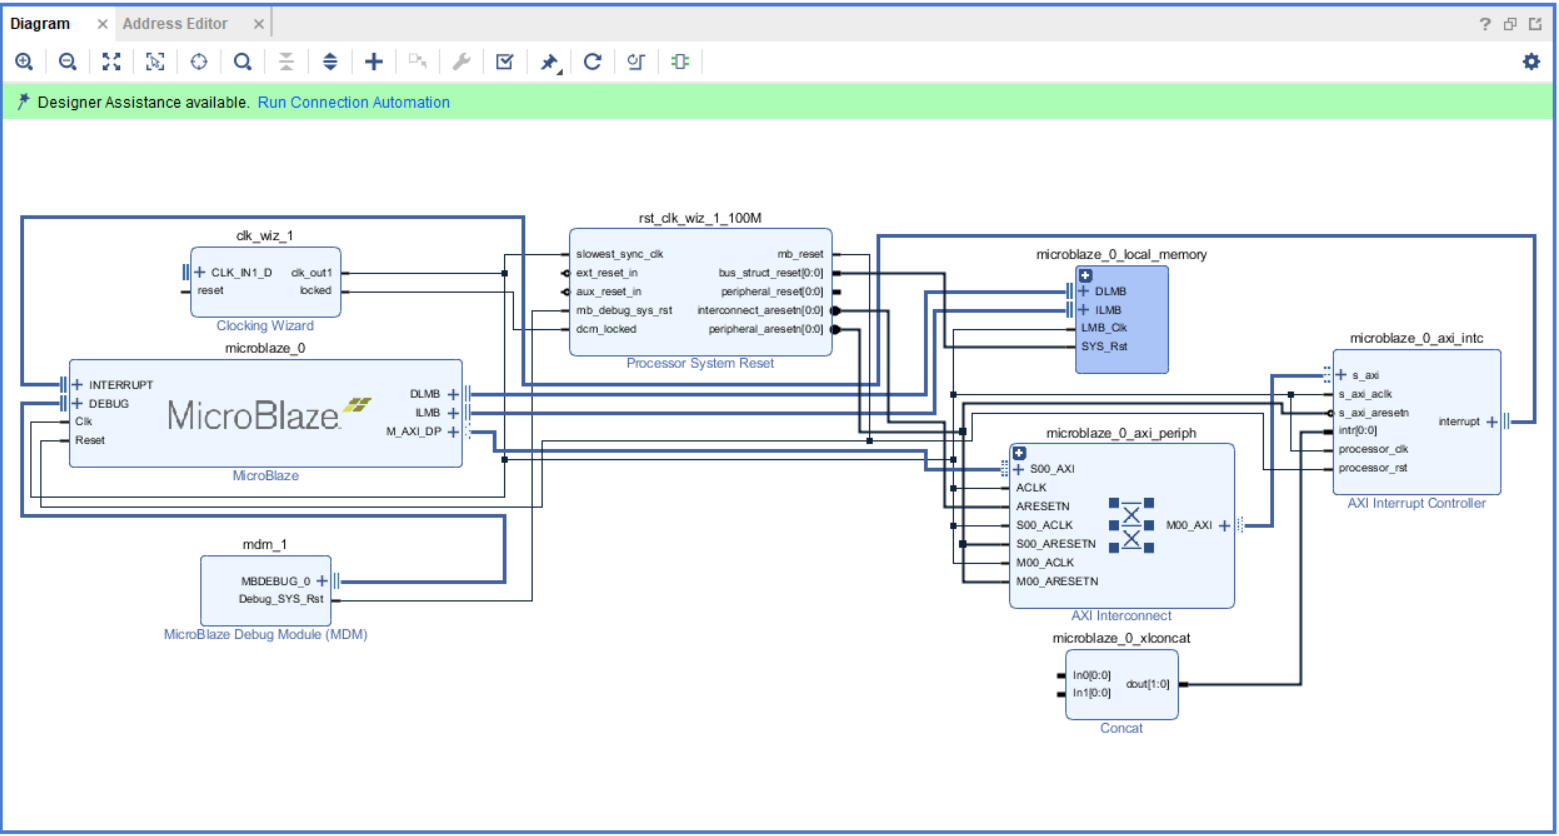
\includegraphics[width=\textwidth]{images/block_design_mb.png}
    \caption{The Block Design after Block Automation}
    \label{fig:block_design_mb}
\end{figure}

The \textit{Block Automation} also added both program and data memory. To see this memory, note the block that was added called \textit{microblaze\_0\_local\_memory} (or something similar). This block isn't actually an IP Core (note the different colour of the block), but a level of hierarchy instantiated in our block design. \textbf{Click} the plus in the corner of this block, or \textbf{double-click} the block, to view the contents of this level of hierarchy. There are a couple of IP Cores here that facilitate access to some local memory for the MicroBlaze. The MicroBlaze uses an interface called \textit{Local Memory Bus}, that needs to be decoded by an \textit{LMB BRAM} controller in order to access the contents of a Block RAM (BRAM) component. BRAMs are a form of memory available on Xilinx FPGAs. Note, the Data and Instructions paths are connected to the same block memory, so they share the same memory space; if you wanted the data and instruction paths to be in different memory spaces, you could add a separate BRAM in this hierarchy.

Finally, \textit{Block Automation} also adds IP Cores to handle the clocks and resets in the system. The \textit{Clock Wizard} IP Core takes a clock from one of the pins of the FPGA and can generate one or more clocks to be used within the FPGA; in our case, a single 100MHz clock is generated for the MicroBlaze and all of the peripherals. The \textit{Processor System Reset} generates separate reset signals for the processor, the peripherals, and the interconnect, according to the AXI standard. We need to make some changes to the clocking configuration, so \textbf{Double click} the \textit{Clocking Wizard} and scroll to the bottom of the first tab. Change the \textit{Source} of the \textit{Primary} input clock to \textbf{Single ended clock capable pin}; the clock supplied to the FPGA will use a single wire instead of a differential signal requiring two wires, which is more often used for very high speed clocks. In the \textit{Output Clocks} tab, change the \textit{Reset Type} to \textbf{Active Low} and Press \textbf{OK}. See Figure~\ref{fig:customize_clock} for reference.

\begin{figure}[h]
    \centering
    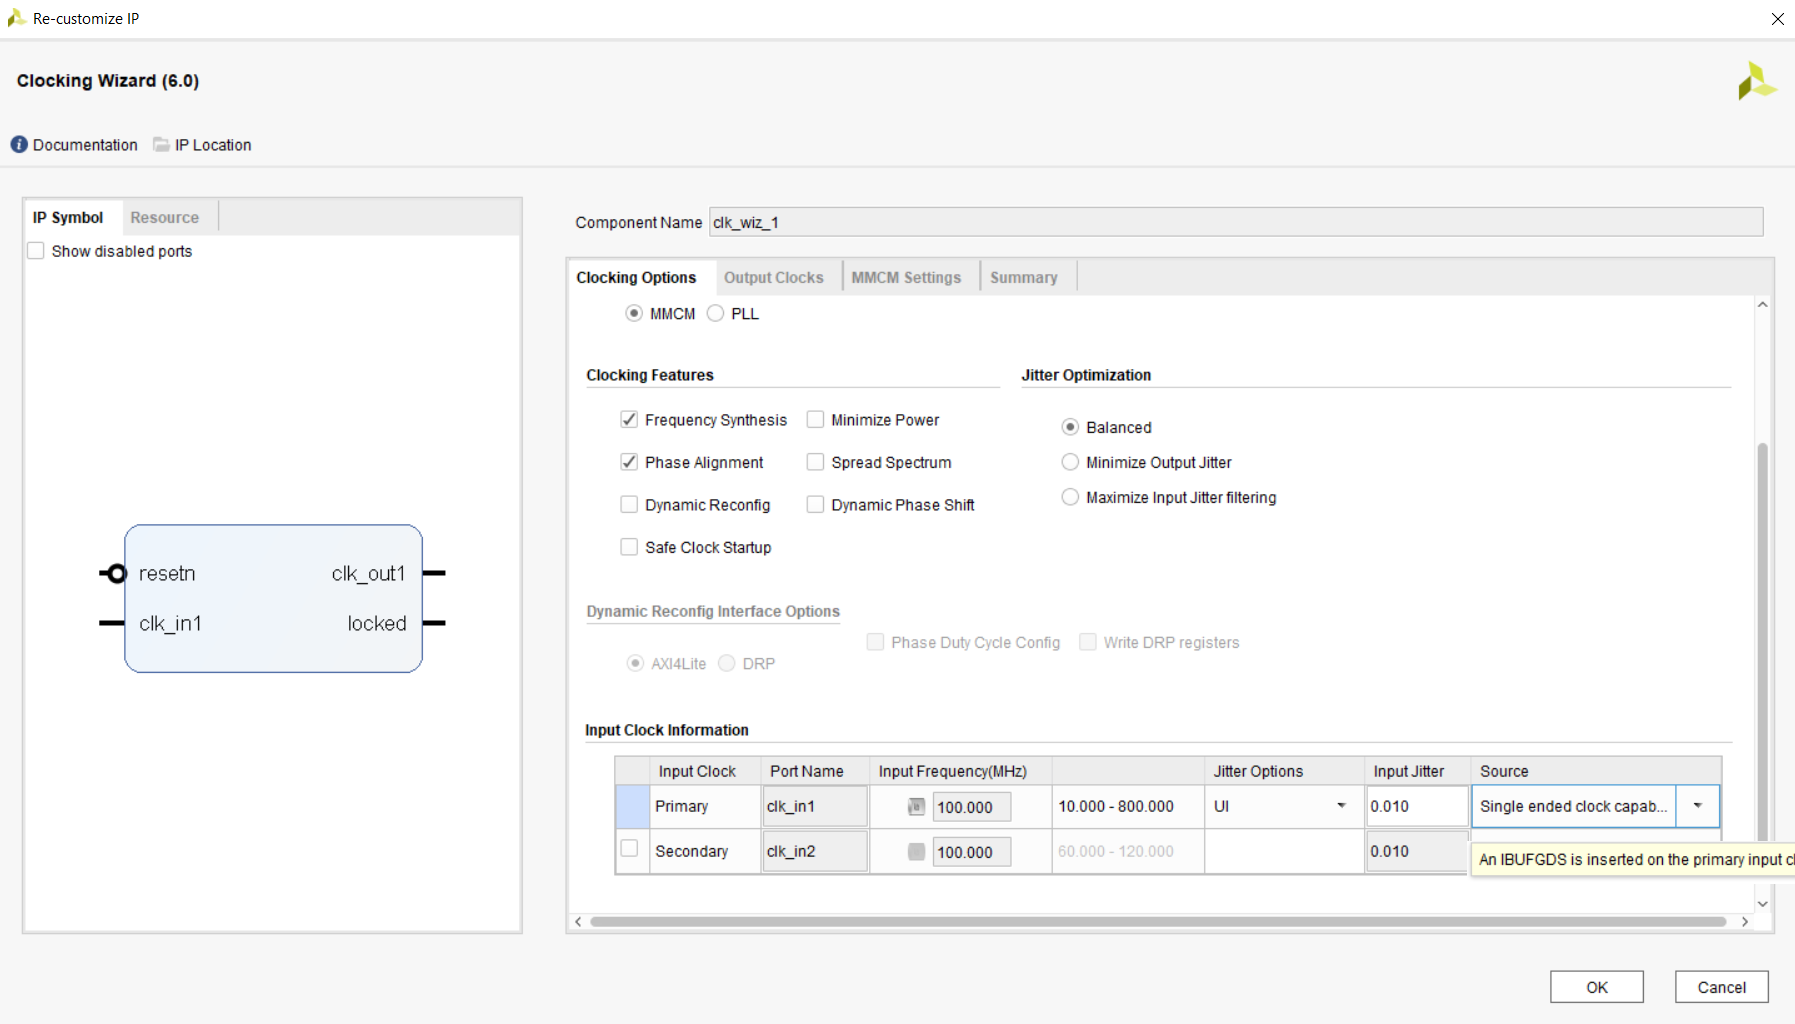
\includegraphics[width=\textwidth]{images/customize_clock.png}
    \caption{Clocking Wizard block customization interface}
    \label{fig:customize_clock}
\end{figure}

The last step we need to do in order to make this a fully functional system is to connect the clock and reset signals to external ports. To do this, we'll use \textit{Connection Automation}, a link to which should have popped up at the top of your block design 
(~\scalerel*{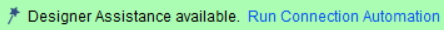
\includegraphics{images/connect_auto_pop.png}}{(}~). Click \textbf{Run Connection Automation} at the top to launch the Connection Automation wizard. \textit{Connection Automation} will allow you to select any unconnected signals and Vivado will try to automatically connect them for you. In our case this includes the \textit{clk} and \textit{resetn} signals of the \textit{Clocking Wizard} and the \textit{ext\_reset\_n} siganl of the \textit{Processor System Reset} core. \textbf{Select} both of the signals for the \textit{Clocking Wizard}, but don't select the \textit{ext\_reset\_n} signal (we'll connect that manually). Click the \textbf{resetn} signal and ensure that \textit{ACTIVE LOW} is selected, and then click \textbf{OK}. See Figure~\ref{fig:conn_auto_clock} for reference.

\begin{figure}[h]
    \centering
    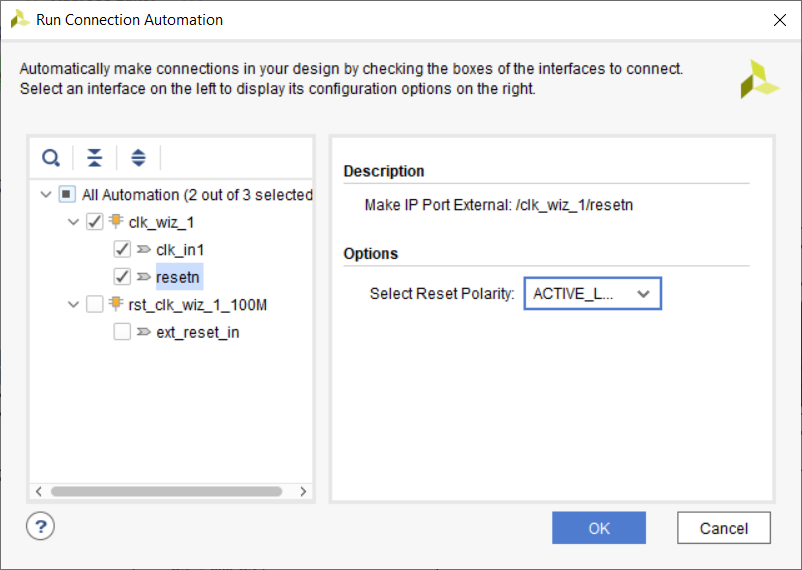
\includegraphics[width=0.9\textwidth]{images/conn_auto_clock.png}
    \caption{Connection automation for the clocking wizard}
    \label{fig:conn_auto_clock}
\end{figure}

The \textit{Connection Automation} should have added two input ports to the design, a clock and a reset port. These ports were automatically connected to the clocking wizard. As a final step, \textbf{click} on the \textit{ext\_reset\_n} signal on the \textit{Process System Reset} IP core when the \textit{pen-like} cursor~(\scalerel*{
\includegraphics{images/connect_pen.png}}{(}) appears and \textbf{drag} the cursor to the newly created reset signal; this will connect the \textit{ext\_reset\_n} signal to the same reset pin we just created. Note, if we had chosen to do \textit{Connection Automation} for the \textit{ext\_reset\_n} signal, it would have created a separate external pin (we want only a signal external reset). We should now have two ports connected to our design as in Figure~\ref{fig:added_reset_conns}.

\begin{figure}[h]
    \centering
    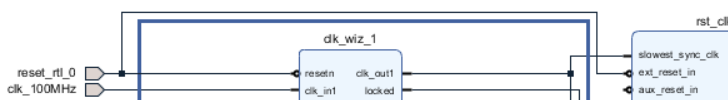
\includegraphics[width=0.9\textwidth]{images/added_reset_conns.png}
    \caption{The ports added to the block design}
    \label{fig:added_reset_conns}
\end{figure}




\section{Adding Peripherals}
\label{sec:add_periph}
We want to add some peripherals to our system to demonstrate that the MicroBlaze can actually interact with other devices and peripherals instantiated within the FPGA or connected to the pins of the FPGA. As a simple example, we'll connect the MicroBlaze system to the switches and LEDs of our board. In addition, we'll add a connection to the UART interface on our board, in order to allow the MicroBlaze to print statements to the console in the Vivado SDK later.

To connect to the LEDs and switches, we need to add AXI GPIO IP cores. GPIO stands for General Purpose I/O, and is used to connect directly to the pins of the FPGA. The AXI GPIO allows this connection to the pins to be accessible from an AXI interface. \textbf{Right click} anywhere in the block diagram, select \textbf{Add IP} and search for and select the  AXI GPIO. Repeat this step so that you have two GPIO blocks in your design. The reason why there are two GPIO blocks is that one of them is for switches and another one is for LEDs so that you can control the LEDs using the switches. Right click one of the GPIO block and click \textbf{Block Properties}. Change the name to \textbf{gpio\_led}. Right click the other GPIO block and click \textbf{Block Properties}. Change the name to \textbf{gpio\_switch}. See Figure~\ref{fig:gpio_prop} for reference.

\begin{figure}[h]
    \centering
    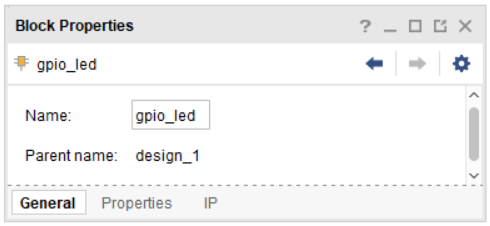
\includegraphics[width=0.5\textwidth]{images/gpio_prop.png}
    \caption{The AXI GPIO block properties window}
    \label{fig:gpio_prop}
\end{figure}

\begin{figure}[!h]
    \centering
    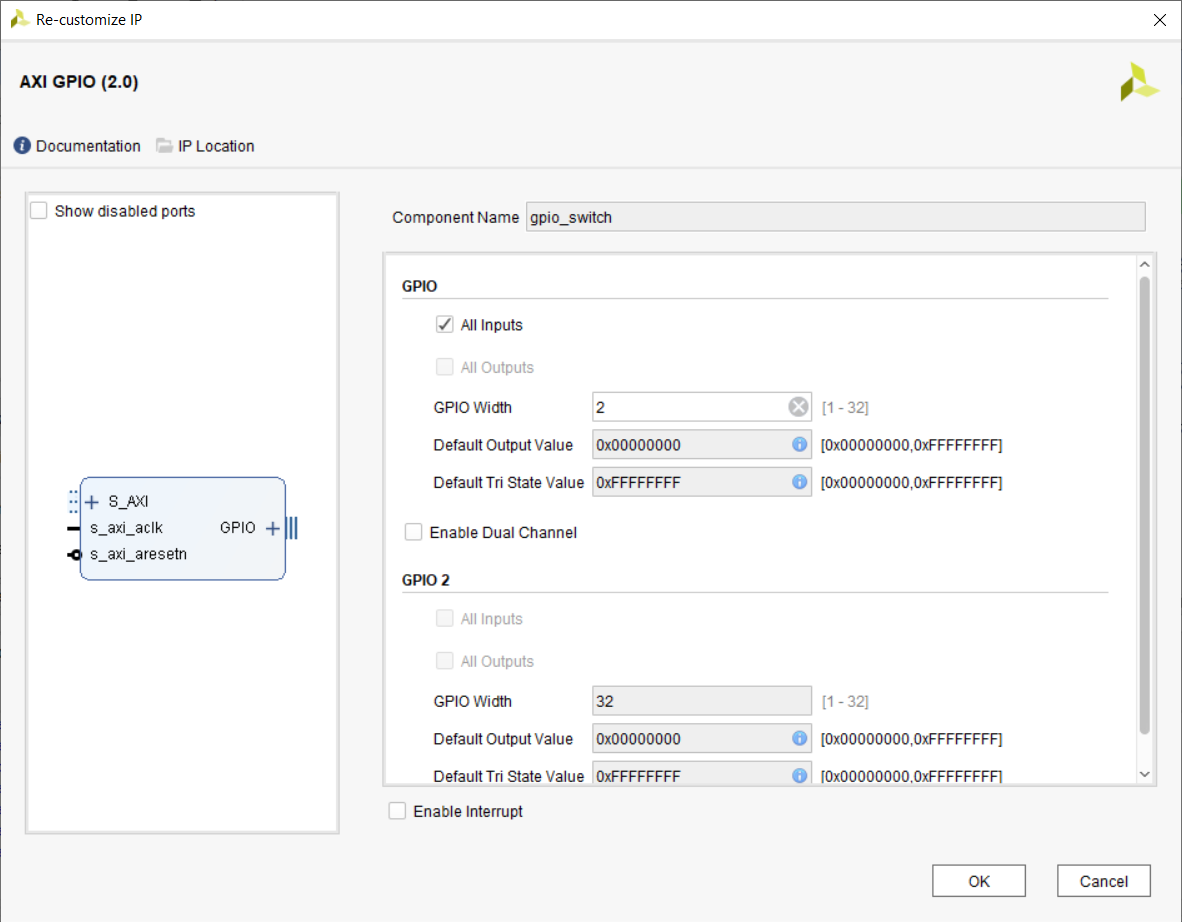
\includegraphics[width=0.9\textwidth]{images/gpio_config.png}
    \caption{The AXI GPIO configuration window}
    \label{fig:gpio_config}
\end{figure}

Now we need to configure and connect our GPIO cores. Double click on \textbf{gpio\_led} to bring up the configuration window. Check the \textbf{All Outputs} checkbox and change the GPIO Width to 2 as we only need to use 2 LEDs for this tutorial. If you need more LEDs, you can change the width to the value you wish. Double click on \textbf{gpio\_switch} block and configure the block to accept two inputs in a similar manner. Note, the switch GPIO should be set to \textit{All Inputs}. See Figure~\ref{fig:gpio_config} for reference. Expand the GPIO port on gpio\_switch by clicking the plus sign. Right click on \textbf{gpio\_io\_i} and choose \textbf{make external}. Expand the GPIO port on gpio\_led by clicking the plus sign. Right click on \textbf{gpio\_io\_o} and choose \textbf{make external}. This last step will allow the GPIO ports to connect to pins on the FPGA. Once the ports have been made external, we should have a connectivity as per Figure~\ref{fig:gpio_connect}.

\begin{figure}[h]
    \centering
    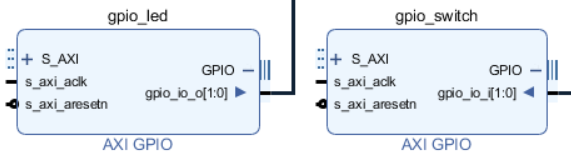
\includegraphics[width=0.6\textwidth]{images/gpio_connect.png}
    \caption{The AXI GPIO connectivity}
    \label{fig:gpio_connect}
\end{figure}

Next, we'll add the AXI Uartlite peripheral to our project. \textbf{Right click} anywhere in the block diagram, select \textbf{Add IP} and search for and select the AXI Uartlite. This core has an interrupt functionality that needs to be connected to our MicroBlaze \textit{Interrupt Controller} in order to function properly. Connect the \textbf{interrupt} signal of the AXI Uartlite to the \textbf{In0} signal of \textit{Concat}, that connects to the interrupt input of the interrupt controller. \textit{Concat} is used to concatenate individual signals into a bus signal. Note that there is one input of the \textit{Concat} block that is not connected and there is no other input to connect to the block. Leaving the unconnected input open will result in critical warnings and ultimately an error when you reach the SDK. There are several ways to deal with this particular situation. To reduce the number of ports, \textbf{double click} on the \textit{Concat} block and
change the number of ports to 1 in the Re-customize IP window. Click \textbf{OK}. We should have a connectivity as per Figure~\ref{fig:uart_connect}.

\begin{figure}[h]
    \centering
    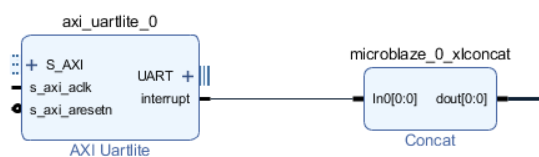
\includegraphics[width=0.6\textwidth]{images/uart_connect.png}
    \caption{The UART Lite connectivity}
    \label{fig:uart_connect}
\end{figure}

To handle the remaining connections we will use connection automation. Click on \textbf{Run Connection Automation} and select
\textbf{All Automation}. This will connect the GPIO and UART controllers to the AXI Interconnect and connect all of the clock and reset signals to the appropriate sources. You should now have a complete system with a MicroBlaze processor, three AXI peripherals, interrupt controller, local memory, debug module and clock and reset generators, as per Figure~\ref{fig:block_design_full}. The \textit{AXI Interconnect} was expanded to add all of the peripherals to the MicroBlaze's memory space. Note, it is often useful to \textbf{right click} and select \textbf{Regenerate Layout} in order to clean up the layout of your blocks.

\begin{figure}[h]
    \centering
    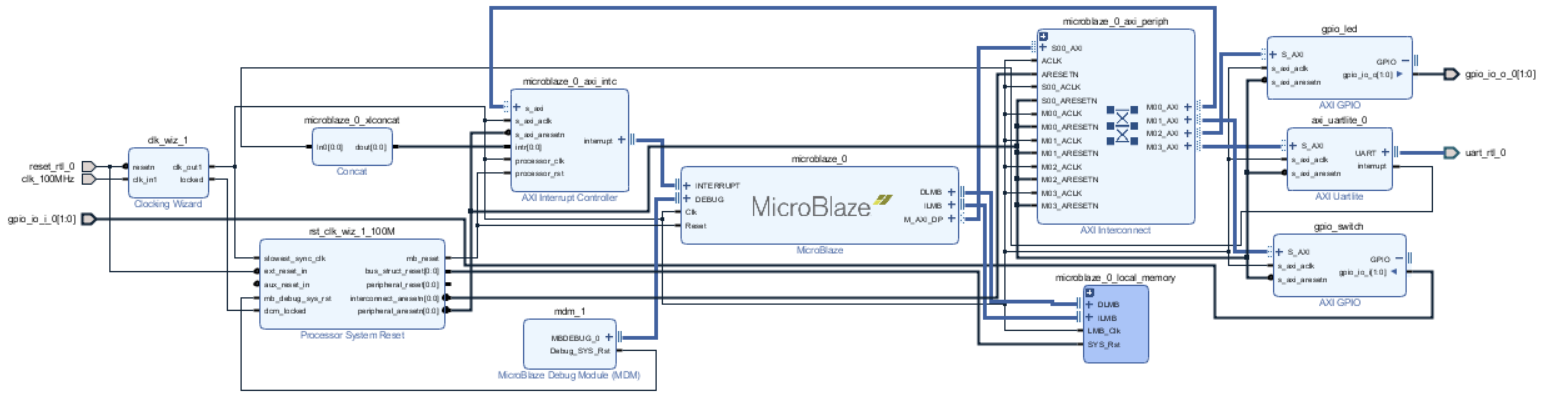
\includegraphics[width=\textwidth]{images/block_design_full.png}
    \caption{The full block design with a MicroBlaze and three peripherals}
    \label{fig:block_design_full}
\end{figure}

An important step in any MicroBlaze system design process is to set the memory-mapping. Note, the \textit{Connection Automation} mapped all of the peripherals for us automatically, but we should still examine it ourselves. Click on the \textbf{Address Editor} tab to examine the address map. This table shows how different peripherals are mapped into the address spaces of different bus masters. In this design, the master is the MicroBlaze soft processor. For instance, notice that the gpio led peripheral can be accessed starting from the address 0x4001\_0000 from the Data port of the MicroBlaze (see Figure~\ref{fig:address_map}). Note, a 64k region was assigned to all of the peripherals, though that size is likely overkill and can be reduced to 4k if you like. The range selected for the BRAMs however is significant, as Vivado uses this range to determine how to size the BRAM inside the block design.

\begin{figure}[h]
    \centering
    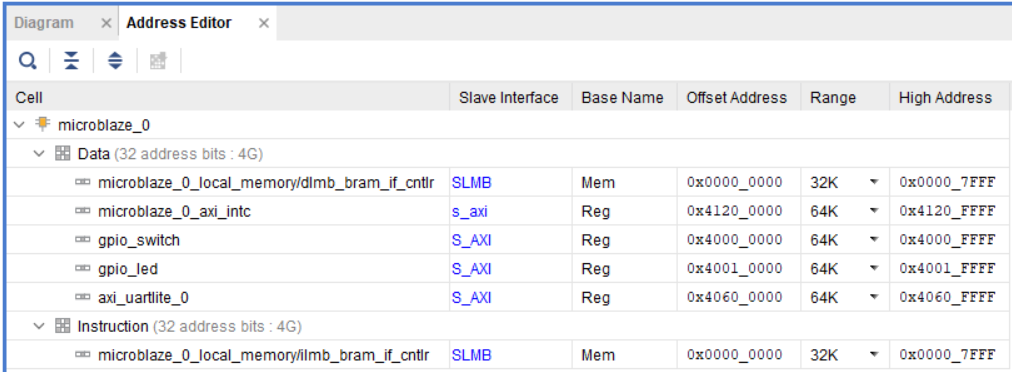
\includegraphics[width=0.9\textwidth]{images/address_map.png}
    \caption{The address map for the data and instruction ports of the MicroBlaze}
    \label{fig:address_map}
\end{figure}

As a finale step, we must validate the design to ensure all of the connections are made and every peripheral is mapped properly. To do this, press the \textbf{Validate Design} button
(\scalerel*{
\includegraphics{images/validate_button.png}}{(})
on the top toolbar in Vivado. If validation is successful, click \textbf{OK}, otherwise check the errors and critical warnings to see what's wrong with the design. Save the block design and then close the block design editor view to return to the \textit{Project Manager} view in Vivado.




\section{Creating a Wrapper and Adding Constraints}
\label{sec:wrap_cons}

In order to use a block design in our project, we have to create an HDL wrapper which instantiates an instance of our block design. The block design itself cannot be the top level module of the project. In the \textit{Sources} pane, click \textbf{Design Sources}. \textbf{Right click} your block design and choose \textbf{Create HDL Wrapper} to wrap your design. A dialog box pops up with some options for the HDL wrapper; the default options are okay, so simply click \textbf{OK}. See Figure~\ref{fig:create_wrapper} for reference. Navigate through the hierarchy of the design in the Hierarchy tab. You will notice that a top-level verilog file was created. As the design flow continues, HDL files will be generated for each block in the IP Integrator design.

\begin{figure}[h]
    \centering
    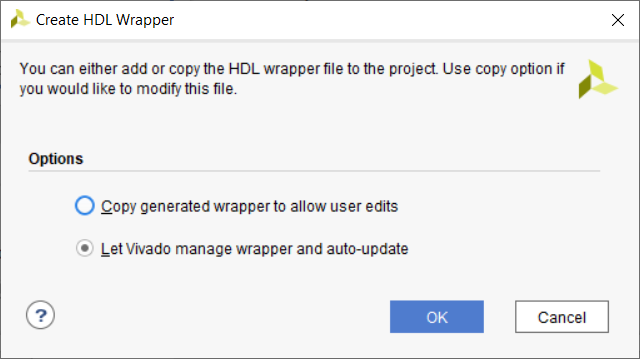
\includegraphics[width=0.7\textwidth]{images/create_wrapper.png}
    \caption{Create HDL wrapper dialog box}
    \label{fig:create_wrapper}
\end{figure}

Open the newly created HDL wrapper by \textbf{double clicking} it in the \textit{Sources} pane. Note that all of the ports that we added to the block design are exposed as top level ports on the verilog wrapper. Within the verilog module, you should see an instance of the block design instantiated. If you want to create your own wrapper, perhaps with some other logic included, this wrapper can be used to determine how to instantiate your block design. The most important feature of the wrapper for the proposes of this tutorial is the name of the top level ports; this is important when creating the constraints file because the names of the ports in the constraints file must match the names in this wrapper.

Open the constraints file you included when you created the project. Verify that the names of all the signals matches the names of the signals in the top level module. As versions of Vivado change, some of these signals may not have the same names as when this tutorial was created. If any of the signal names don't match between the wrapper and the constraints file, change the constraints file to match the verilog wrapper. The contents of the constraints file as of the making of this document are displayed in Figure~\ref{fig:constraints_file}. Now that we have a valid constraints file, we can proceed to build the project, we need to run \textbf{Synthesis}, followed by \textbf{Implementation}, and the \textbf{Generate Bitstream} steps. Note, if you run only the \textbf{Generate Bitstream} step, Vivado will run through \textbf{Synthesis} and \textbf{Implementation} automatically.

\begin{figure}[!h]
\centering
\begin{minted}
[
frame=lines,
framesep=2mm,
baselinestretch=1.2,
bgcolor=white,
fontsize=\footnotesize,
linenos,
breaklines,
]
{tcl}
## Clock signal
set_property -dict { PACKAGE_PIN E3    IOSTANDARD LVCMOS33 } [get_ports { clk_100MHz }];
create_clock -add -name sys_clk_pin -period 10.00 -waveform {0 5} [get_ports {clk_100MHz}];

## Reset (CPU_RESET)
set_property -dict { PACKAGE_PIN C12   IOSTANDARD LVCMOS33 } [get_ports { reset_rtl_0 }];

##Switches
set_property -dict { PACKAGE_PIN J15   IOSTANDARD LVCMOS33 } [get_ports { gpio_io_i_0[0] }];
set_property -dict { PACKAGE_PIN L16   IOSTANDARD LVCMOS33 } [get_ports { gpio_io_i_0[1] }];

## LEDs
set_property -dict { PACKAGE_PIN H17   IOSTANDARD LVCMOS33 } [get_ports { gpio_io_o_0[0] }];
set_property -dict { PACKAGE_PIN K15   IOSTANDARD LVCMOS33 } [get_ports { gpio_io_o_0[1] }];

##USB-RS232 Interface
set_property -dict { PACKAGE_PIN C4    IOSTANDARD LVCMOS33 } [get_ports { uart_rtl_0_rxd }];
set_property -dict { PACKAGE_PIN D4    IOSTANDARD LVCMOS33 } [get_ports { uart_rtl_0_txd }];
\end{minted}
\vspace{-0.7cm}
\caption{Constraints file for the project}
\label{fig:constraints_file}
\end{figure}



\newpage
\section{Hello World Program in Vivado SDK}
\label{sec:hello_sdk}

After generating the bitstream, click on \textbf{File} and choose \textbf{Export}, then choose \textbf{Export Hardware}. Make sure you check \textbf{Include bitstream} (see Figure~\ref{fig:export_hw}). If the option is gray, make sure to click \textbf{Open Implemented Design} under the \textit{Implementation} section of the \textit{Flow Navigator} and repeat the export step. Then, click \textbf{File} and select \textbf{Launch SDK}, which will launch the Vivado SDK program. Note, Vivado SDK can take some time to load the hardware, so be patient.

\begin{figure}[h]
    \centering
    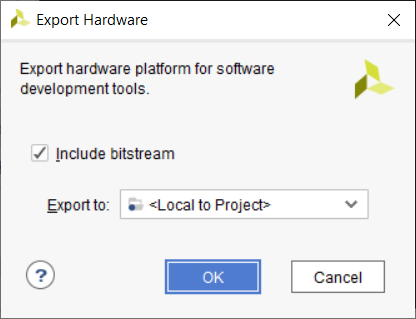
\includegraphics[width=0.4\textwidth]{images/export_hw.png}
    \caption{Export hardware with include bitstream checked}
    \label{fig:export_hw}
\end{figure}

After the SDK first launches, double click \textbf{system.hdf} to see the information created when you exported the hardware in the previous step. You'll see a description of the peripherals connected to the MicroBlaze processor as well as the memory-map we created using the \textit{Address Editor} (see Figure~\ref{fig:export_hdf}). If there are missing peripherals, or the memory-map doesn't match that which we created in the block design, the hardware must have been exported incorrectly; sometimes this is the case when we update the the block design but forget to re-export the hardware in Vivado.

\begin{figure}[h]
    \centering
    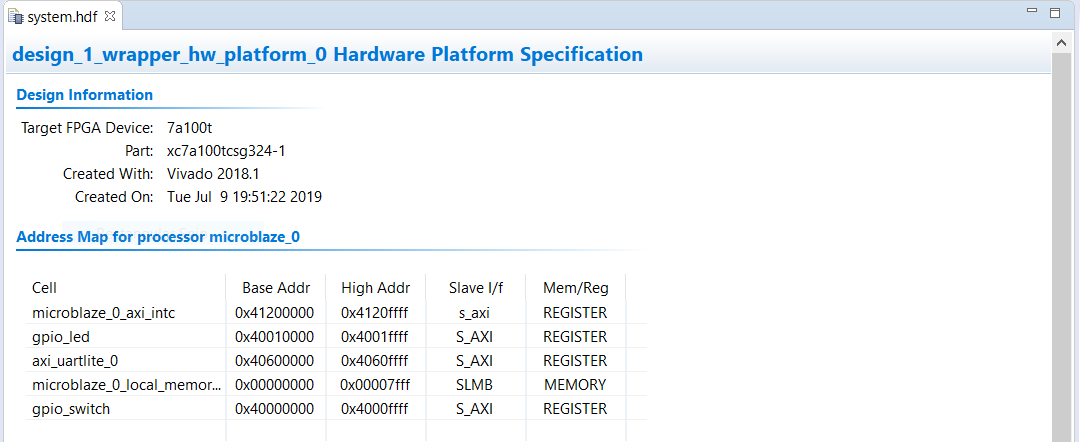
\includegraphics[width=0.9\textwidth]{images/export_hdf.png}
    \caption{Export hardware in Vivado SDK}
    \label{fig:export_hdf}
\end{figure}

Vivado SDK provides some template programs to help us get started with programming for the MicroBlaze system. We will be creating a \textit{Hello World} application. Select \textbf{File $\rightarrow$ New $\rightarrow$ Application Project}. Enter some \textbf{Project name} and choose the \textit{OS Platform} to be \textbf{standalone}. Click \textbf{Next}. Choose \textbf{Hello World} as your template and click \textbf{Finish}. See Figure~\ref{fig:new_app_hello} for reference.

\begin{figure}[h]
    \centering
    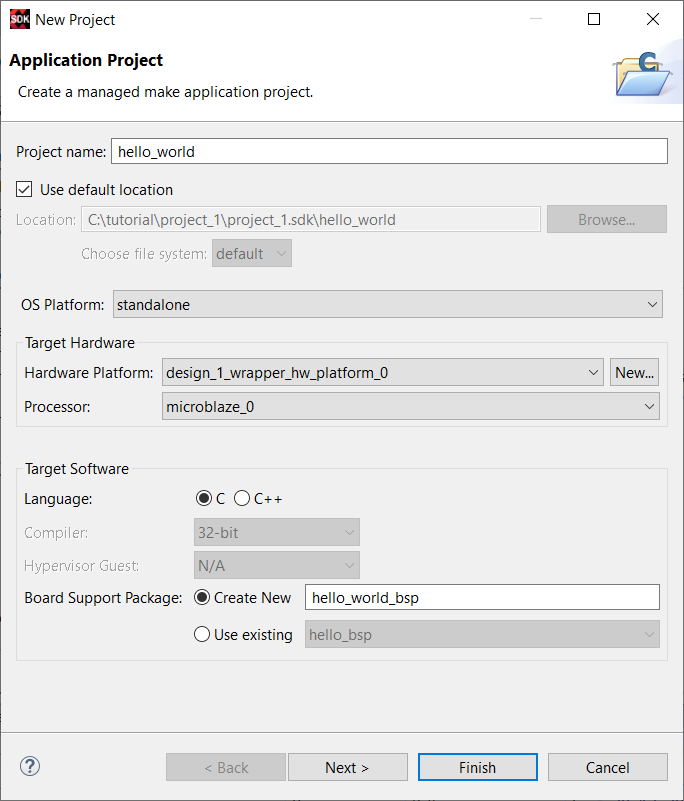
\includegraphics[width=0.7\textwidth]{images/new_app_hello.png}
    \caption{Creating a new application in Vivado SDK}
    \label{fig:new_app_hello}
\end{figure}


The created application is opened in the Vivado SDK IDE, with a listing of source and include files on the left hand side. expand both the new application folder, and the folder with ending \textit{\_bsp} to see the folder structure of the application. In the \textit{src} folder of your application directory, you should now see a file called \textit{helloworld.c}, along with files called \textit{platform.c}, \textit{platform.h}, and \textit{platform\_config.h}. The main function is defined in the \textit{helloworld.c} file, so \textbf{double click} that file to open it up and view the contents. You should see a program which calls functions \textit{init\_platform()} and \textit{cleanup\_platform()} at the beginning and end of the program, with some functionality included within. These two functions are defined in the \textit{platform.c} file, and call other functions that themselves are defined in the \textit{platform.c} file, or perhaps in some include files from the aforementioned \textit{\_bsp} directory. The \textit{\_bsp} directory, which stands for \textit{Board Support Package}, contains drivers for the peripherals included in your design and some common Xilinx functionalities. You may want to take a look at some of these files if you're curious. These two functions setup the platform for us to use and should always be included in any project.

\newpage
\textbf{Connect} your board to the computer and turn it on. Click \textbf{Xilinx Tools $\rightarrow$ Program FPGA} to program your board with the generated bitstream. If you have multiple boards connected, make sure to select the correct board by clicking \textbf{Select...} beside the \textit{Device} field, otherwise the \textbf{Auto Detect} option should be fine. The bitstream should be automatically selected in this window. Click \textbf{Program} to start programming the board. See Figure~\ref{fig:program_fpga} for reference. Note, this will program the board with the MicroBlaze system we created.

\begin{figure}[h]
    \centering
    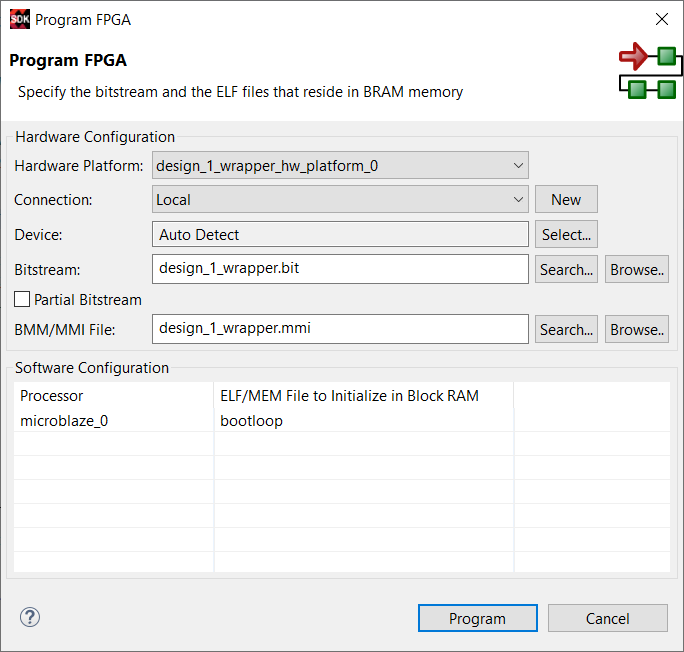
\includegraphics[width=0.68\textwidth]{images/program_fpga.png}
    \caption{The program FPGA dialog in Vivado SDK}
    \label{fig:program_fpga}
\end{figure}

To run the application on the board, click on \textbf{Run $\rightarrow$ Run Configurations} to create a new run configuration. Choose \textbf{Xilinx C/C++ application(GDB)} and then click the \textbf{New} button
(\scalerel*{
\includegraphics{images/new_run_button.png}}{(})
to create a new launch. You should now see the interface depicted in Figure~\ref{fig:new_run_config}. Open the \textbf{Application} tab and click \textbf{Browse} next to the \textit{Project Name} entry box, select your newly created hello world program (based on the name you assigned it earlier). You will notice that the application file is automatically selected under the \textit{Debug} folder. In the \textit{Summary} section above, click the \textbf{checkbox} in the \textit{Download} column of the application. Click \textbf{Apply} to save the run but do not run the application just yet. Click \textbf{Close}.

\begin{figure}[!h]
    \centering
    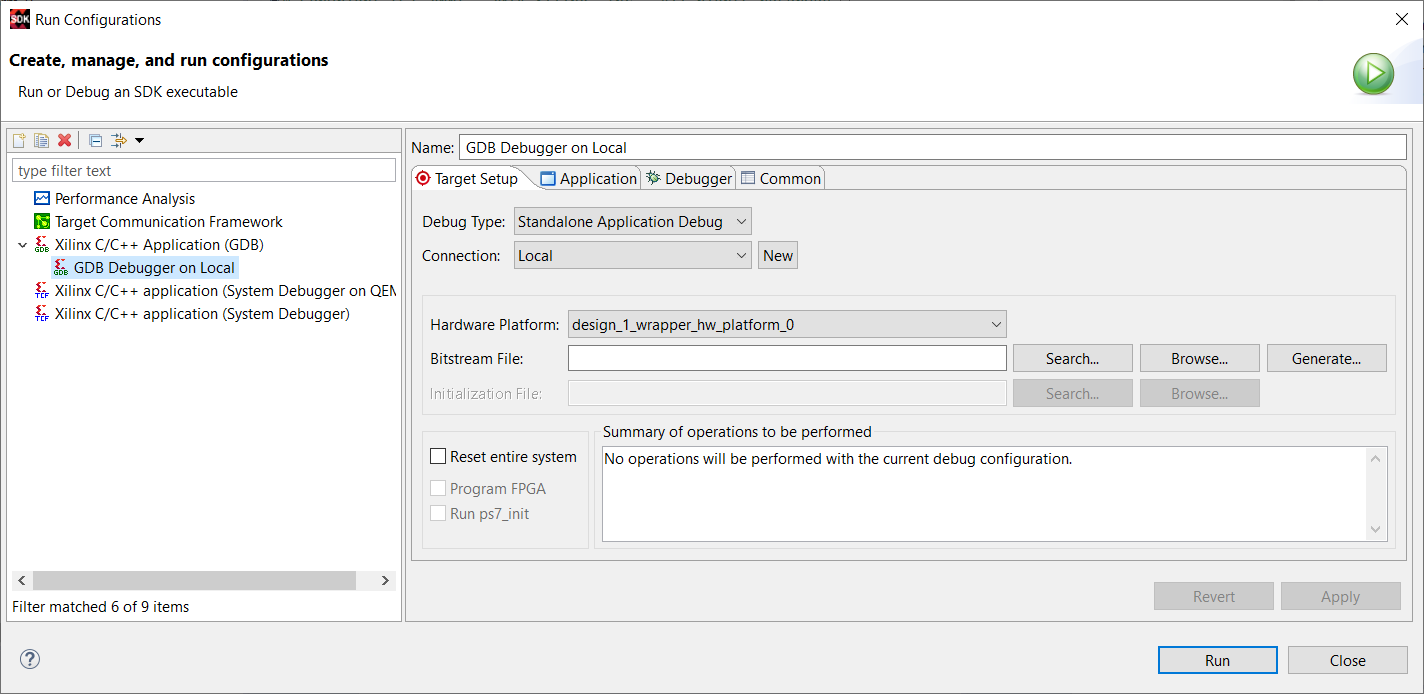
\includegraphics[width=\textwidth]{images/new_run_config.png}
    \caption{Creating a new run in Vivado SDK}
    \label{fig:new_run_config}
\end{figure}

\newpage
To see the output of the print statements in our program, we must connect to the UART port of the board. To do this, select the \textbf{SDK Terminal} tab in the console window at the bottom of Vivado SDK. Now click the \textbf{Plus} button 
(\scalerel*{
\includegraphics{images/sdk_conn_button.png}}{(})
to add a new connection. A dialog will pop up to specify the details of the connection (see Figure~\ref{fig:sdk_conn_dialog}). On Windows machines, the \textit{Port} field should be a drop down list containing the terminal devices connected to the computer; \textbf{select} the device corresponding to the board's UART connection. On Linux machines, you must enter the device file name corresponding to the terminal device in this field (e.g. /dev/ttyUSBx where x is the number corresponding to the connection). For Linux, you must add yourself to the \textit{dialout} group before performing this step. Set the \textit{Baud Rate} to \textbf{9600} and click \textbf{OK}. If you don't know the port number of the board, you can try different options until you find the correct one, though be careful not to send characters to some other terminal device attached to your computer. If testing different port numbers, remember to disconnect from the previous port before connecting to a new port. Any output from the UART port of the board will be displayed in this \textit{SDK Terminal} tab.

\begin{figure}[h]
    \centering
    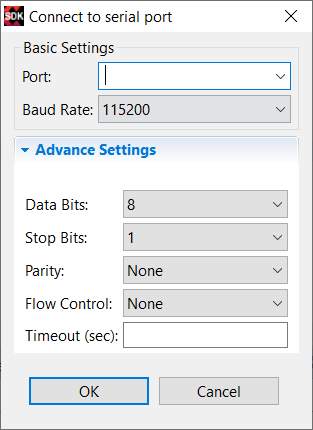
\includegraphics[width=0.4\textwidth]{images/sdk_conn_dialog.png}
    \caption{New SDK terminal connection dialog}
    \label{fig:sdk_conn_dialog}
\end{figure}

Re-open the \textbf{Run Configurations} window and select the run you recently created listed under \textit{Xilinx C/C++ application(GDB)}. Click \textbf{Run} to run the application. If the board is found successfully, there should be no errors. Check the \textit{SDK Terminal} tab to ensure that the \textit{Hello World} text was printed correctly.




\section{Program to Access the GPIOs}
\label{sec:prog_gpio}

Open the \textit{helloworld.c} file and modify its contents to match that in Figure~\ref{fig:gpio_app}. This program defines two volatile global pointers to the LED and switch GPIO addresses; accesses to these addresses will access the registers of the AXI GPIO cores in our block design. The macros \textit{XPAR\_GPIO\_LED\_BASEADDR} and \textit{XPAR\_GPIO\_SWITCH\_BASEADDR} are defined in a file called \textit{xparameters.h}, which is found in the \textit{include} folder of the board support package directory. Make sure to check that file to ensure your macros have the same name (if they differ, please change them in the modified \textit{helloworld.c} program to match those given in \textit{xparameters.h}). In this application, the infinite while loop keeps checking the value of the switches and assigns them to the LEDs. This way you can control the LEDs from the switches.

\begin{figure}[!h]
\centering
\begin{minted}
[
frame=lines,
framesep=2mm,
baselinestretch=1.2,
bgcolor=white,
fontsize=\footnotesize,
linenos,
breaklines,
]
{c}
#include <stdio.h>
#include "platform.h"
#include "xil_printf.h"
#include "xparameters.h"

volatile unsigned int* led = (unsigned int*) XPAR_GPIO_LED_BASEADD;
volatile unsigned int* swt = (unsigned int*) XPAR_GPIO_SWITCH_BASEADD;

int main()
{
    init_platform();

    print("Hello World\n\r");
    
    while(1)
    {
        *led = *swt;
    }

    cleanup_platform();
    return 0;
}
\end{minted}
\vspace{-0.7cm}
\caption{Modified Hello World application using GPIOs}
\label{fig:gpio_app}
\end{figure}

Re-open the \textbf{Run Configurations} window and select the run you recently created listed under \textit{Xilinx C/C++ application(GDB)}. Click \textbf{Run} to run the application. Try flipping the switches on the board and see what happens to the LEDs. Note, while it may seem that the changes to the LED is instantaneous, in actuality there is some time between changes to the switches and the corresponding changes to the LED values. This delay isn't perceivable since the MicroBlaze is running at 100MHz.

To see this delay, we need to insert some breakpoints. Click \textbf{Run $\rightarrow$ Debug Configurations} to bring up the debug configurations. The run configuration we created earlier should already exist as a debug configuration in this view, \textbf{select it} on the left side and click \textbf{Debug}. A prompt will come up telling you that Vivado SDK will open the \textit{Debug perspective}, click \textbf{Yes}. The window view that appears is the gdb debugger view in Vivado SDK (see Figure~\ref{fig:gdb_view}). Variables and Breakpoints are listed in the pane on the right side, and the program contents and outline are shown in the lower portion of the figure.

\begin{figure}[h]
    \centering
    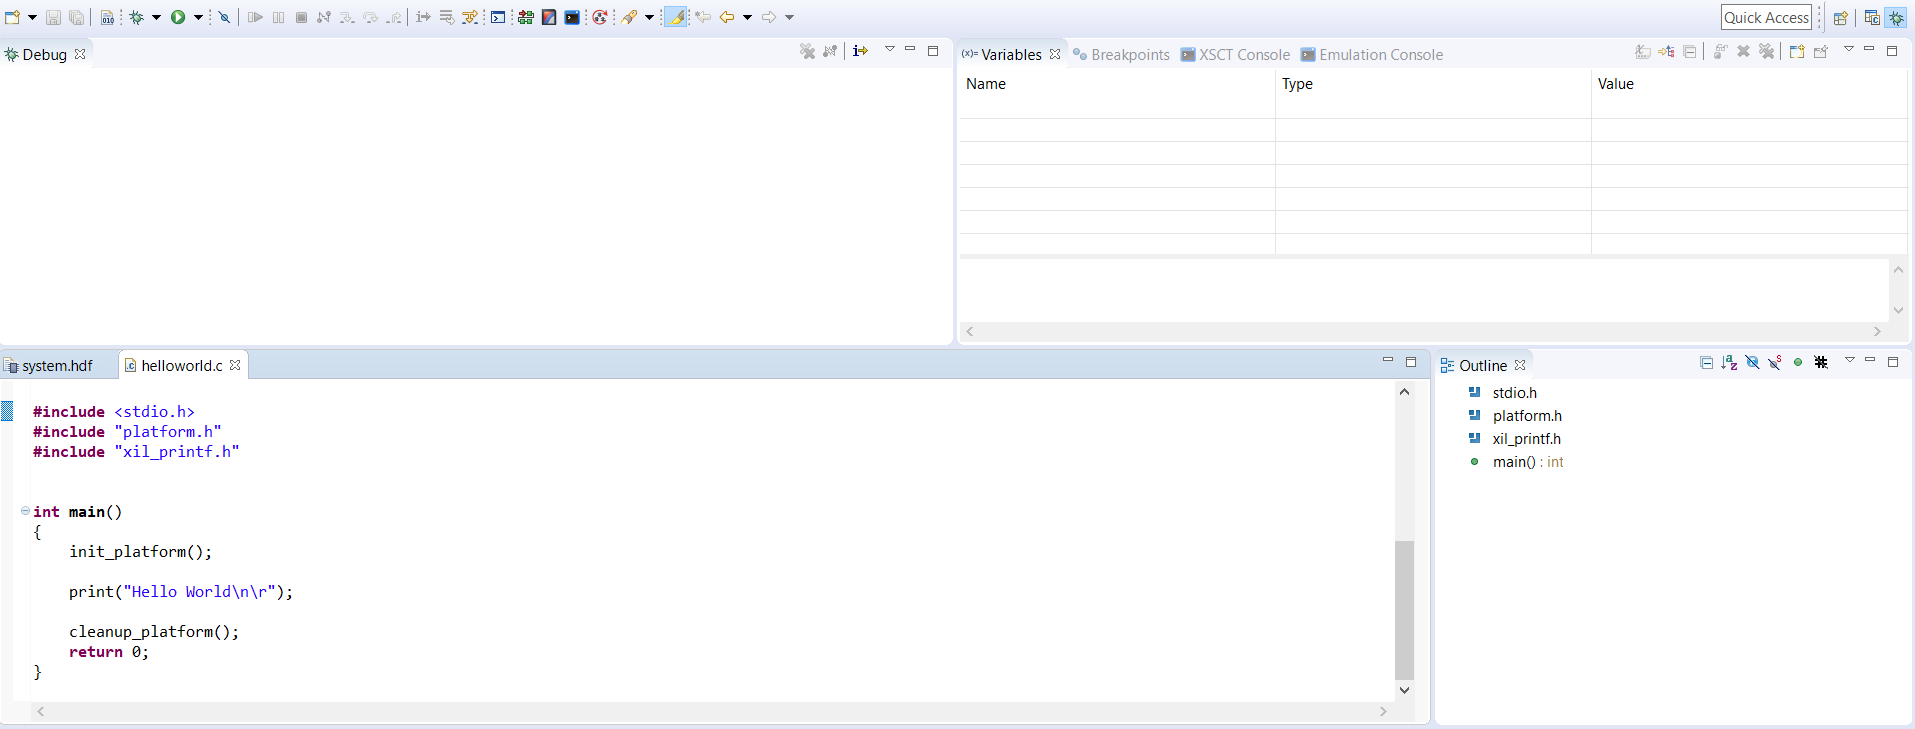
\includegraphics[width=\textwidth]{images/gdb_view.png}
    \caption{GDB debugging view in Vivado SDK}
    \label{fig:gdb_view}
\end{figure}

\newpage
You can add breakpoints by \textbf{double clicking} to the left of the line of code before which you'd like the program to stop, i.e. in the margins of the code. Insert a breakpoint on line 17 (refer to Figure~\ref{fig:gpio_app}). Press the \textbf{Resume} button
(\scalerel*{
\includegraphics{images/gdb_resume_button.png}}{(})
to advance the program to the next break (note, if the program didn't break at the beginning of the main function by default, you will have to stop the program first by pressing the \textbf{Stop} button
\scalerel*{
\includegraphics{images/gdb_stop_button.png}}{(}). Change the switch values with the program stopped and observer that the LEDs do not change correspondingly. Click \textbf{Resume} again to see the LED values update again. We can thus confirm that the LED values are indeed being changed by the software running on the MicroBlaze. The GDB debugger is a useful tool to help debug your applications running on the MicroBlaze system.




\section{Summary}
\label{sec:summary}
The Vivado IP Integrator flow can be used to easily create complex hardware systems, including soft-processor systems with MicroBlaze processors. The project was created with a block design, and a full MicroBlaze system was built in that block design with a number of Xilinx IP cores, including three peripherals. The system was built and a bitstream was generated. The Hardware was exported and Vivado SDK was launched, reading the exported hardware. Example \textit{Hello World} and \textit{GPIO} applications were made and run on the MicroBlaze. The GDB debugger was also used to insert breakpoints into the software and step through the code.



%\newpage
%S\printbibliography

\end{document}
